\begin{figure}[tbp]
\begin{center}
\includegraphics[width=0.48\textwidth]{figure/k3pd_k3pv_z1.eps}
\end{center}
\vspace{-0.7cm}
\caption{
    Illustrating weights of different scales after integration for redshift 1.
    (Top) The density variance $2\pi^2\Delta_\delta^2\equiv k^3P_\delta$. 
    (Bottom) The velocity variance $2\pi^2\Delta_{v_z}^2\equiv k^3P_{v_z}$. 
    Red lines: indicate the most essential modes for generating kSZ signal in 
    $\ell~500-3000$.
}
\label{fig:k3v}
\end{figure}

\begin{figure}[tbp]
\begin{center}
\includegraphics[width=0.48\textwidth]{figure/cmb_21cm.eps}
\end{center}
\vspace{-0.7cm}
\caption{
    (Top) Relative strength of angular powerspectrum between primary CMB, Planck noise in 217 GHz band, and kSZ effect in redshift 1 and 2.
    (Bottom) Demonstrate available modes of density contrasts obtained 
    in realistic 21cm Intensity Mapping experiments, 
    with resolution of CHIME and high foregrounds. 
    $P_{21cm}$ is the remaining density powerspectrum after noise substraction; 
    $P_\delta$ indicates the powerspectrum of a comtact density field.
}
\label{fig:cmb_21cm}
\end{figure}

%Since actual sky surveys can only resolve structures of certain scales, 
%it is essential to understand which scales contribute most to the kSZ signals. 
To understand what role each scale plays in generating kSZ signal, we write Eq.(\ref{eq:ksz}) in Fourier space. 

The finite box size of $1200$ Mpc only has notable influence on modes with $k\lesssim0.005$. 
It is safe to assume 
minus infinity to plus infinity 
integration on $z$ direction for small scale modes. 

Moreover, the term $a(z)H(z)f(z)$ in Eq.(\ref{eq:v}) does not vary much in one box, we assume it to be a constant for simplicity. 
Then the Fourier transformation is just the $k_z=0$ mode of the momentum 
$p_\parallel(\bm{k})$ in Fourier space. 
\begin{eqnarray}
    \label{eq:thetak}
    \Theta(\bm{\ell})&\equiv&\Theta({k}_x\chi,{k}_y\chi,0)\\
    &\propto&\int 
    d^3k^\prime\delta(\bm{\ell}/\chi-\bm{k}_\perp^\prime,k_\parallel^\prime) v_z(\bm{k^\prime})\nonumber
%    \xrightarrow[region]{linear}&\int& 
%d^3k^\prime\delta({\bm{k}}_\perp-\bm{k}_\perp^\prime,k_\parallel^\prime)\delta(\bm{k}^\prime)\frac{k_z^\prime}{k'^2}
    \end{eqnarray}
An essential feature of Eq.(\ref{eq:thetak}) is that
in transverse plane, density and velocity field of different scales are multiplied together, 
 while in parallel direction, only $\delta$ and $v_z$ of 
 identical $k_z$ are coupled together.  

The relative strength of $|\delta(\bm{k})|$ and $|v_z(\bm{k})|$ in different scales 
are implied in Fig.\ref{fig:k3v}. 
and also implicit at Eq.(\ref{eq:v}), 
The velocity field contributes almost dominantly from large scale structures, 
leaving little contribution from $k_z>0.2 h/Mpc$, $k_\perp> 0.02 h/Mpc$. 
%ignoring the vast k modes in this region. 
This makes it roughly an ellipitical selection functions in the convolution
---
It selects $\delta$ with similar range of $k_z$ and $k_\perp\sim(\ell/\chi-0.01)$ h/Mpc.  
Actually, the sharper $|v(\bm{k})|$ is 
the more it ressembles a Delta Function peaked at 
$(k_\perp,k_\parallel)=(0.01,0.1)$ h/Mpc. 
Then 
\begin{eqnarray}
    \Theta(\bm{l}) &\propto& \int\, 
    d^3k^\prime\delta(\bm{\ell}/\chi-\bm{k}_\perp^\prime,k_\parallel^\prime) 
    \delta^D(0.01,0.1) \\
    &\sim& \delta(\ell/\chi-0.01,0.1).
\end{eqnarray}
Therefore, when generating kSZ signals, 
it is crucial to have large scale modes for $v_z$. 
However, which scales matter most for $\delta(\bm{k})$ 
depends on the $\ell$ we look at.  

To decide the targeted $\ell$ range, 
many factors needs to be taken into account:  
the strength of the primary CMB, facility limits and 
other fluctuations on CMB such as thermal SZ effect\cite{} and CMB lensing\cite{}.
Consider using Planck \cite{Planck2015} data 
in the 217 GHz band, where the tSZ signal vanishes, 
we demonstrate the angular powerspectrum of primary CMB, 
facility noises (detailed calculations in Section VI), 
and kSZ of redshift 1 and 2 
in Fig.\ref{fig:CMB}. 
Only in the range of $\ell \sim 500-3000$, 
there is a chance for us to distinguish the kSZ signal.  

Therefore, in Fig.\ref{fig:k3v}, we roughly sketch the essential modes 
for $v_z(\bm{k})$ and $\delta(\bm{k})$ 
in red lines. 
Linearly, velocity field of a certain scale only relates to 
identical scale of density field, see Eq.(\ref{eq:v}). 
Therefore, an ideal cross correlation density field should be intact in both regions. 

Note: all the demonstration figures are towards redshift 1, 
however, there is only slight difference  
in redshift 2, 
which should not influence the qualitive analysis.
